\documentclass[10pt]{beamer}

\usepackage[T2A]{fontenc}
\usepackage[utf8]{inputenc}
\usepackage[russian,english]{babel}

\usefonttheme[onlymath]{serif}

\usetheme[progressbar=frametitle]{metropolis}
\usepackage{appendixnumberbeamer}

\usepackage{booktabs}
\usepackage[scale=2]{ccicons}

\usepackage{pgfplots}
\usepgfplotslibrary{dateplot}

\usepackage{xspace}
\newcommand{\themename}{\textbf{\textsc{metropolis}}\xspace}
\newcommand{\TODO}[1]{\textbf{\textcolor{red}{TODO: #1}}}

\date{}
\author{Екатерина Тузова}


\usepackage{gensymb}

\title{Лекция 8}
\subtitle{Нейронные сети}

\begin{document}	

\section{Разбор летучки}

\frame{\titlepage}

\begin{frame}\frametitle{Нейрон}
	\begin{figure}[htbp]
	  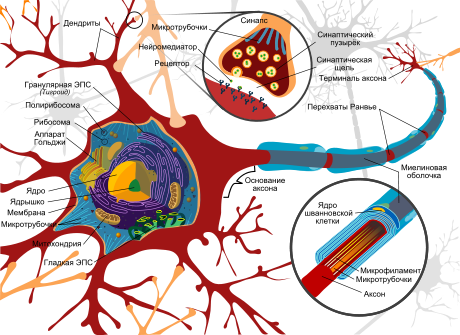
\includegraphics[height=200pt, keepaspectratio = true]{images/neuron}   
	\end{figure}
\end{frame}

\begin{frame}\frametitle{Линейная модель нейрона}
	Модель МакКаллока-Питтса:\\
	$f_j: X \rightarrow R, \hspace{10mm} j = 1,\dots, n$ — числовые признаки\\
	$a(x,w) = \sigma(\langle w, x_i \rangle) = \sigma(\sum\limits_{j=1}^n w_j f_j(x) - w_0)$\\
	где $w_0, w_1, \dots,w_n \in R$ -- веса признаков\\
	$\sigma(s)$ -- функция активации (например, $\sign$)
	
	\begin{figure}[htbp]
	  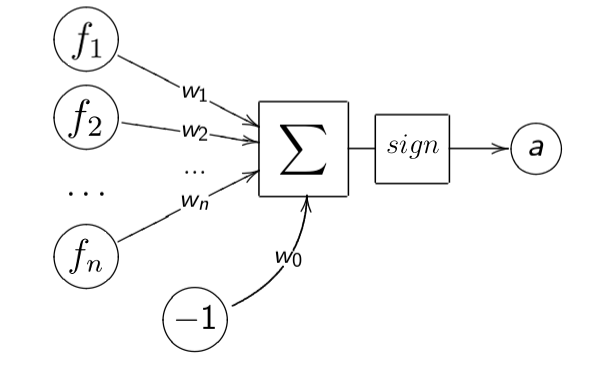
\includegraphics[height=100pt, keepaspectratio = true]{images/neuron-scheme}   
	\end{figure}
\end{frame}

\begin{frame}\frametitle{Линейные алгоритмы классификации и регрессии}
	Задача классификации: \\
	$Y = \left\{ \pm1 \right\}, \hspace{10mm} a(x,w) = \sign \langle w, x_i \rangle $\\
	$Q(w;X^l) = \sum\limits_{i=1}^l \mathcal{L} (\langle w, x_i\rangle y_i) \rightarrow \min\limits_w$\\
\end{frame}

\section{Какой класс функций можно реализовать нейроном?}

\begin{frame}\frametitle{Нейронная реализация логических функций}
	\begin{figure}[htbp]
	  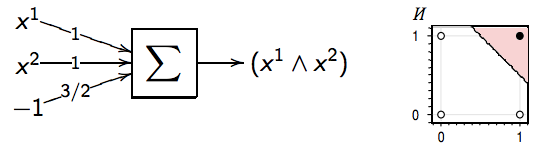
\includegraphics[height=60pt, keepaspectratio = true]{images/OR}   
	\end{figure}
	
	\begin{figure}[htbp]
	  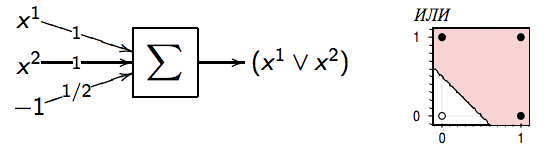
\includegraphics[height=60pt, keepaspectratio = true]{images/AND}   
	\end{figure}
\end{frame}

\begin{frame}\frametitle{Нейронная реализация логических функций}
	Функции И, ИЛИ, НЕ от бинарных переменных $x_1$ и $x_2$:\\
	$$x_1 \wedge x_2 = x_1 + x_2 - \frac{3}{2} > 0$$\\
	$$x_1 \vee x_2 = x_1 + x_2 - \frac{1}{2} > 0$$\\
	$$\neg x_1 = -x_1 + \frac{1}{2}> 0$$
\end{frame}

\begin{frame}\frametitle{Логическая функция XOR}
	\begin{figure}[htbp]
	  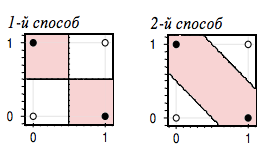
\includegraphics[height=150pt, keepaspectratio = true]{images/XOR}   
	\end{figure}
\end{frame}

\begin{frame}\frametitle{Логическая функция XOR}
	Функция $x_1 \oplus x_2 = [x_1 \neq x_2]$ не реализуема одним нейроном.\\
	
	Два способа реализации:\\
	\begin{enumerate}[--]
		\item Добавлением нелинейного признака:\\
		$x_1 \oplus x_2 = [x_1 + x_2 + 2x_1x_2 - \frac{1}{2} > 0]$
		\item Сетью (двухслойной суперпозицией) функций И, ИЛИ, НЕ:\\
		$x_1 \oplus x_2 = [(x_1 \vee x_2) - (x_1 \wedge x_2) - \frac{1}{2} > 0]$
		\end{enumerate}
\end{frame}

\begin{frame}\frametitle{Логическая функция XOR}
	\begin{figure}[htbp]
	  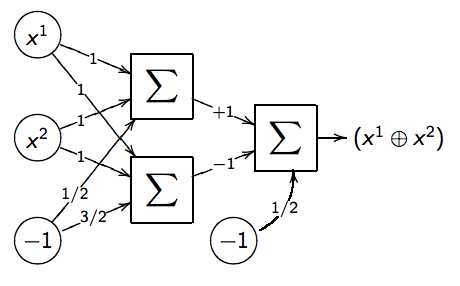
\includegraphics[height=150pt, keepaspectratio = true]{images/XOR1}   
	\end{figure}
\end{frame}

\begin{frame}\frametitle{Любую ли функцию можно представить нейросетью?}
	\begin{enumerate}[--]
		\item Двухслойная сеть в $\left\{0, 1 \right\}^n$ позволяет реализовать произвольную булеву функцию.
		\item Двухслойная сеть в $\mathbb{R}^n$ позволяет отделить произвольный выпуклый многогранник.
		\item Трёхслойная сеть $\mathbb{R}^n$ позволяет отделить произвольную многогранную область, не обязательно выпуклую, и даже не обязательно связную.
		\item С помощью линейных операций и одной нелинейной функции активации $\sigma$ можно приблизить любую непрерывную функцию с любой желаемой точностью
	\end{enumerate}
\end{frame}

\begin{frame}\frametitle{Практические рекомендации}
	\begin{enumerate}[--]
    	\item Двух-трёх слоёв обычно достаточно.
	  \item Можно достраивать нейроны в произвольных местах сети по необходимости.
	\end{enumerate}
\end{frame}

\begin{frame}\frametitle{Многослойная нейронная сеть}
	Пусть $Y = \mathbb{R}^M$, два слоя в сети.\\
	
	\begin{figure}[htbp]
	  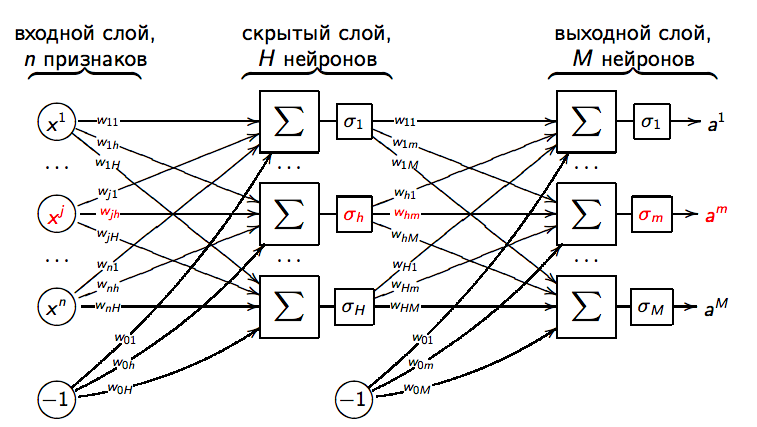
\includegraphics[height=150pt, keepaspectratio = true]{images/neural_network}   
	\end{figure}
\end{frame}

\begin{frame}\frametitle{Многослойная нейронная сеть}
	\begin{figure}[htbp]
	  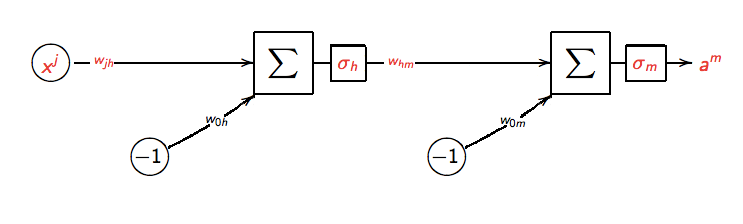
\includegraphics[height=100pt, keepaspectratio = true]{images/neural_network1}   
	\end{figure}
\end{frame}

\begin{frame}\frametitle{Стохастический градиент}
  Задача минимизации суммарных потерь:\\
  ${Q}(\mathbf{w}) = \sum\limits_{i=1}^l \mathcal{L}(w, x_i, y_i) \rightarrow \min\limits_w$ \\
  \begin{algorithmic}[1]
    \Function{stochastic\_gradient}{$X^l$, $\alpha$, $\eta$}
     \State Перемешать данные в $X^l$
     \State Инициализировать $w$, ${Q}(w)$
     \State ${Q}(\mathbf{w}) = \sum\limits_{i=1}^l \mathcal{L}(\langle \mathbf{w}, \mathbf{x_i} \rangle y_i)$
     \MRepeat [пока $Q$ и/или $w$ не стабилизируются] 
       \State Взять $x_i$ из $X^l$
       \State Потеря: $\varepsilon_i = \mathcal{L}(w, x_i, y_i)$
       \State Градиентный шаг: $w =  w - \alpha \triangledown \mathcal{L}(w, x_i, y_i)$
       \State Оценить $Q = (1-\eta)Q + \eta \varepsilon_i$
     \EndRepeat
    \EndFunction
  \end{algorithmic}  
\end{frame}

\section{Сколько операций потребуется для вычисления градиента в точке?}

\begin{frame}\frametitle{Идея}
  \alert{Идея}: Сохранять некоторые промежуточные результаты в узлах сети.
\end{frame}

\begin{frame}\frametitle{Задача дифференцирования суперпозиции функций}
	Выходные значения $a^m(x_i)$, $m = 1,\dots,M$ на объекте $x_i$:\\
	$$a^m(x_i) = \sigma_m (\sum\limits_{h=0}^H w_{hm} u^h(x_i)), \hspace{5mm} u^h(x_i) = \sigma_h (\sum\limits_{j=0}^n w_{jh} f_j(x_i))$$\\
	Возьмем $\mathcal{L}_i(w)$ -- средний квадрат ошибки:\\
	$$\mathcal{L}_i(w) = \frac{1}{2} \sum\limits_{m=1}^M (a^m(x_i) - y_i^m)^2$$\\
	Промежуточная задача: найти частные производные\\
	$$\frac {\partial \mathcal{L}_i(w)}{\partial a^m} \hspace{5mm} \frac {\partial \mathcal{L}_i(w)}{\partial u^h}$$
\end{frame}

\begin{frame}\frametitle{Быстрое вычисление градиента}
  Ошибка на выходном слое:	
	$$\frac{\partial \mathcal{L}_i(w)}{\partial a^m} = a^m (x_i) - y_i^m = \varepsilon^m_i$$ 
	
	Ошибка на скрытом слое:	
	$$\frac{\partial \mathcal{L}_i(w)}{\partial u^h} = \sum\limits_{m=1}^M (a^m(x_i) - y_i^m) \sigma'_m w_{hm} = \sum\limits_{m=1}^M \varepsilon^m_i \sigma'_m w_{hm} = \varepsilon^h_i$$
	$\varepsilon_i^h$ вычисляется по $\varepsilon_i^m$, если запустить сеть «задом наперёд»:\\
	
	\begin{figure}[htbp]
	  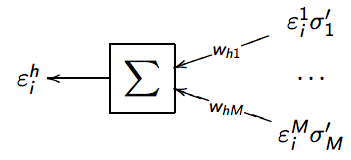
\includegraphics[height=50pt, keepaspectratio = true]{images/backpropagation}   
	\end{figure}

\end{frame}

\begin{frame}\frametitle{Быстрое вычисление градиента}
	Теперь, имея частные производные $\mathcal{L}_i(w)$ по $a^m$ и $u^h$, легко выписать градиент $\mathcal{L}_i(w)$ по весам $w$.\\
	\bigbreak
	\pause
	\alert{Вопрос}: как?
\end{frame}

\begin{frame}\frametitle{Быстрое вычисление градиента}
	$$\frac {\partial \mathcal{L}_i(w)}{\partial w_{hm}} = \frac {\partial \mathcal{L}_i(w)}{\partial a^m} \frac {\partial a^m}{\partial w_{hm}} = \varepsilon^m_i \sigma'_m u^h(x_i), \hspace{50mm}$$ $$m = 1,\dots,M, \hspace{2mm} h = 0,\dots, H$$\\
	
	$$\frac {\partial \mathcal{L}_i(w)}{\partial w_{jh}} = \frac {\partial \mathcal{L}_i(w)}{\partial u^h} \frac {\partial u^h}{\partial w_{jh}} = \varepsilon_i^h \sigma'_h f_j(x_i), \hspace{50mm}$$ $$h = 1,\dots,H, \hspace{2mm} j = 0,\dots, n$$ \\
\end{frame}

\begin{frame}\frametitle{Алгоритм обратного распространения ошибки}
  \begin{algorithmic}[1]
    \Function{stochastic\_gradient}{$X^l \subset \mathbb{R}^n \times \mathbb{R}^M$, $H$, $\alpha$, $\eta$}
     \MRepeat [пока $Q$ не стабилизируются] 
       \State Взять $x_i$ из $X^l$
       \State 	$\begin{cases}
	\hspace{5mm} u^h_i = \sigma_h (\sum\limits_{j=0}^J w_{jh} x_i^j), \hspace{4mm} h = 1, \dots, H\\
	\hspace{5mm} a^m_i = \sigma_m (\sum\limits_{h=0}^H w_{hm} u_i^h), \hspace{4mm} \varepsilon_i^m = a_i^m - y_i^m, \hspace{4mm} m = 1, \dots, M\\
	\hspace{5mm} \mathcal{L}_i = \sum\limits_{m=1}^M (\varepsilon_i^m)^2\\
	\end{cases}$\\
	$\begin{cases} \hspace{5mm} \varepsilon_i^h = \sum\limits_{m=1}^M \varepsilon_i^m \sigma'_m w_{hm}, \hspace{4mm} h = 1, \dots, H\end{cases}$\\
	$\begin{cases} \hspace{5mm} w_{hm} = w_{hm} - \alpha \varepsilon_i^m \sigma'_m u_i^h, \hspace{4mm} h = 0, \dots, H, \hspace{4mm} m = 1, \dots, M\\
	\hspace{5mm} w_{jh} = w_{jh} - \alpha \varepsilon_i^h \sigma'_h x_i^j, \hspace{4mm} j = 0, \dots, n, \hspace{4mm} h = 1, \dots, H\\
	\hspace{5mm} Q = (1 - \eta)Q + \eta \mathcal{L}_i \end{cases}$
     \EndRepeat
    \EndFunction
  \end{algorithmic}  
  
\end{frame}

\begin{frame}\frametitle{Особенности}
	\begin{enumerate}[<+->]
	\item[+] Эффективность: градиент вычисляется за время, сравнимое со временем вычисления самой сети
	\item[+] Легко обобщается на любые $\sigma$, $\mathcal{L}$
	\item[+] Возможно динамическое (потоковое) обучение
	\item[+] На сверхбольших выборках не обязательно брать все $x_i$
	\item[+] Возможность распараллеливания
	\bigbreak
	\item[--] Возможна медленная сходимость
	\item[--] Застревание в локальных минимумах
	\item[--] Проблема переобучения
	\item[--] Подбор комплекса эвристик
	\end{enumerate}
\end{frame}


\begin{frame}\frametitle{Стандартные эвристики для метода SG}
	Применимы все те же эвристики, что и в обычном SG.\\
	\bigbreak
	\pause
	Напомните.
\end{frame}

\begin{frame}\frametitle{Стандартные эвристики для метода SG}
	\begin{itemize}[<+->]
		\item Инициализация весов
		\item Порядок предъявления объектов
		\item Оптимизация величины градиентного шага
		\item Регуляризация (сокращение весов)
	\end{itemize}
\end{frame}

\begin{frame}\frametitle{Новые проблемы}
	\begin{itemize}[<+->]
		\item Выбор функций активации в каждом нейроне
		\item Выбор числа слоёв и числа нейронов;
		\item Выбор значимых связей;
	\end{itemize}
\end{frame}

\begin{frame}\frametitle{Ускорение сходимости}
	\begin{itemize}[<+->]
		\item Тщательный подбор начального приближения
		\item Адаптивный градиентный шаг
		\item Метод сопряжённых градиентов и chunking -- разбиение суммы $Q(w) = \sum\limits_{i=1}^l \mathcal{L}_i(w)$ на блоки
	\end{itemize}
\end{frame}

\begin{frame}\frametitle{Начальное приближение}
	Нейроны настраиваются как отдельные линейные алгоритмы:
	\begin{itemize}
		\item либо по случайной подвыборке $X' \subseteq X^l$
		\item либо по случайному подмножеству входов
		\item либо из различных случайных начальных приближений
	\end{itemize}
	Tем самым обеспечивается различность нейронов.
\end{frame}

\begin{frame}\frametitle{Оптимизация структуры сети}
	Динамическое наращивание сети.\\
	\begin{itemize}[<+->]
		\item Обучение при заведомо недостаточном числе нейронов $H$
		\item После стабилизации  $Q(w)$ -- добавление нового нейрона и его инициализация путём обучения
		\item Снова итерации BackProp
	\end{itemize}
	\vspace{5mm}
	Противоположная идея -- прореживание сети.
\end{frame}

\begin{frame}\frametitle{Специальные нейронные сети}
	Большинство используемых на сегодняшний день методов придуманы в 80-х.\\
	Почему их снова стали использовать?\\
	\begin{enumerate}[--]
		\item Большие вычислительные возможности (в том числе
		распределенные вычисления)
		\item Большие объемы данных
		\item Новые методы предобучения, новые архитектуры
	\end{enumerate}
\end{frame}

\begin{frame}\frametitle{Как было раньше?}
	Ученые придумывали признаки. На них обучали классификатор.\\
	
	\begin{figure}[htbp]
	  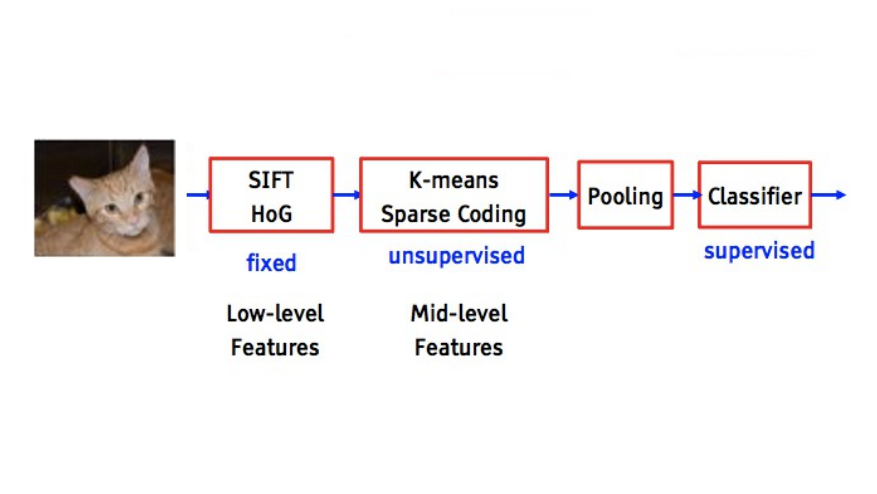
\includegraphics[height=150pt, keepaspectratio = true]{images/old_approach}   
	\end{figure}
\end{frame}

\begin{frame}\frametitle{Deep learning}
  Извлечение признаков во время обучения.\\

	\begin{figure}[htbp]
	  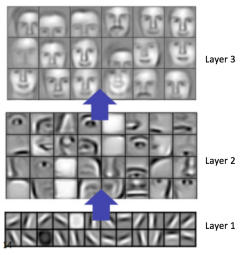
\includegraphics[height=150pt, keepaspectratio = true]{images/deep_learning}   
	\end{figure}
\end{frame}

\begin{frame}\frametitle{Сверточные нейросети}
	Архитектура сети выбирается таким образом, чтобы заложить в нее априорные знания из предметной области:\\
	\begin{enumerate}[--]
		\item Пиксель изображения сильнее связан с соседними пикселями (локальная корреляция)
		\item Объект может встретиться в любой части изображения (инвариантность к перемещению)
	\end{enumerate}
\end{frame}

\begin{frame}\frametitle{Локально-связанный слой}
	Закладываем в архитектуру сети априорное знание о том, что
	соседние пиксели изображения сильнее связаны между собой.\\
	
	\begin{figure}[htbp]
	  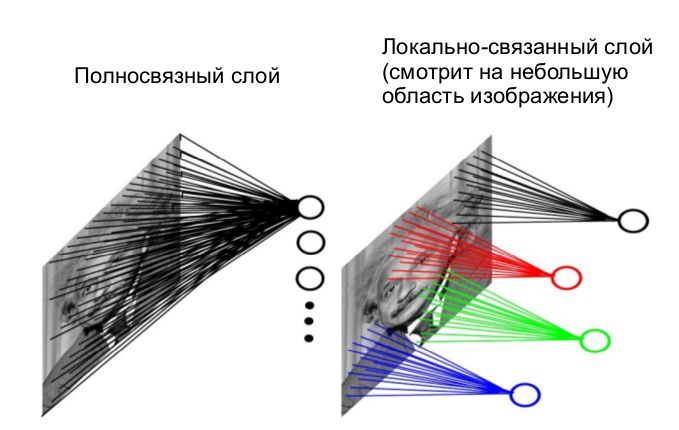
\includegraphics[height=150pt, keepaspectratio = true]{images/local_layer}   
	\end{figure}
\end{frame}

\begin{frame}\frametitle{Инвариантность к перемещению}
	Операция свертки.\\
	\begin{figure}[htbp]
	  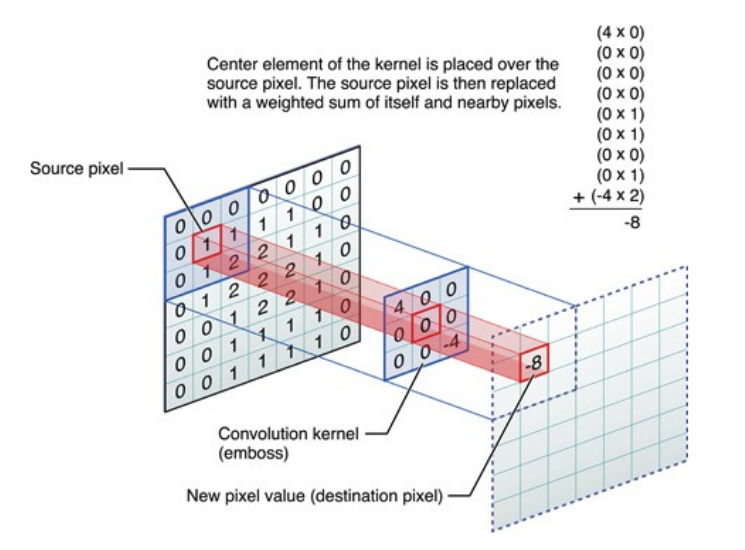
\includegraphics[height=200pt, keepaspectratio = true]{images/conv}   
	\end{figure}
\end{frame}

\begin{frame}\frametitle{Инвариантность к перемещению}
	\begin{figure}[htbp]
	  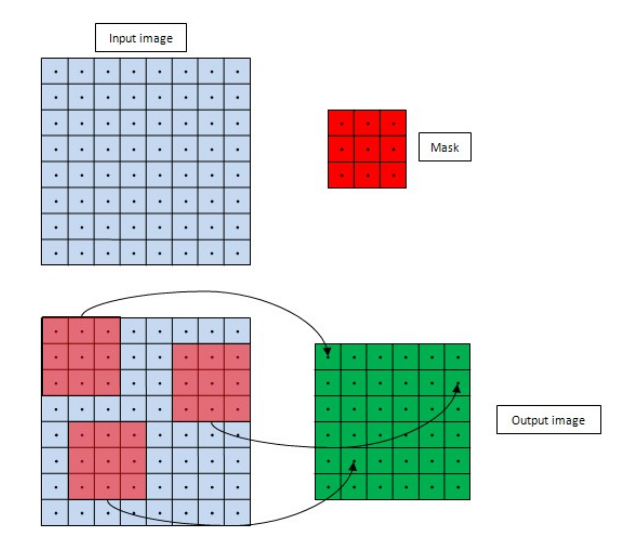
\includegraphics[height=200pt, keepaspectratio = true]{images/conv2}   
	\end{figure}
\end{frame}

\begin{frame}\frametitle{Простейшая свертка}
	\begin{figure}[htbp]
	  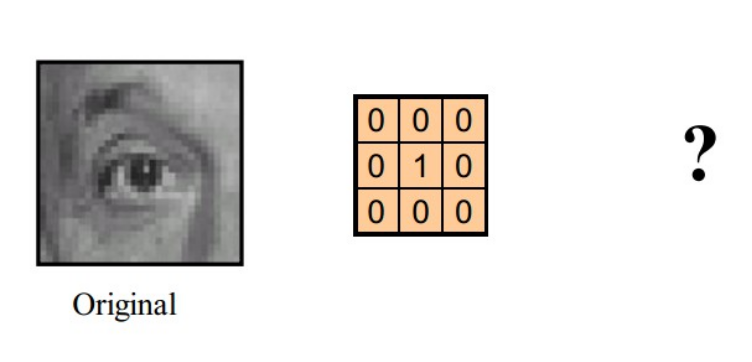
\includegraphics[height=150pt, keepaspectratio = true]{images/conv_easy}   
	\end{figure}
\end{frame}

\begin{frame}\frametitle{Простейшая свертка}
	\begin{figure}[htbp]
	  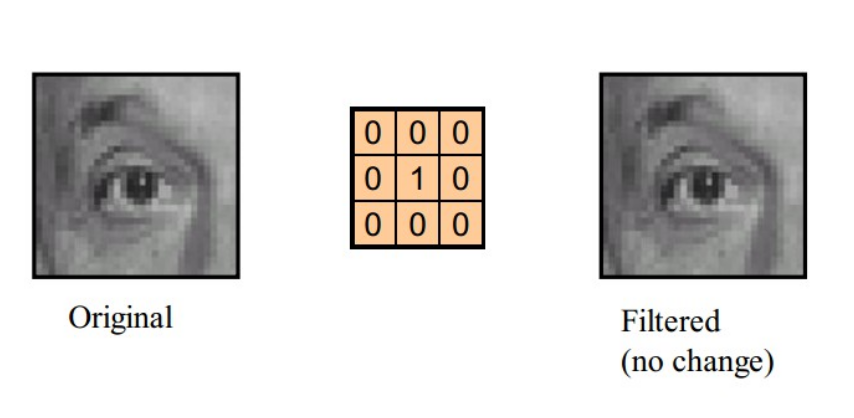
\includegraphics[height=150pt, keepaspectratio = true]{images/conv_easy2}   
	\end{figure}
\end{frame}

\begin{frame}\frametitle{Простейшая свертка}
	\begin{figure}[htbp]
	  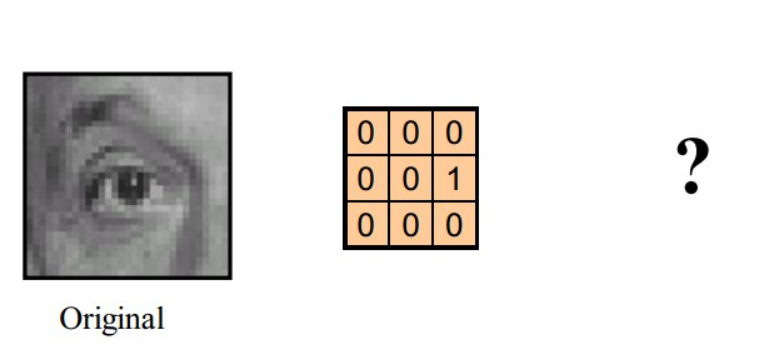
\includegraphics[height=150pt, keepaspectratio = true]{images/conv_easy3}   
	\end{figure}
\end{frame}

\begin{frame}\frametitle{Простейшая свертка}
	\begin{figure}[htbp]
	  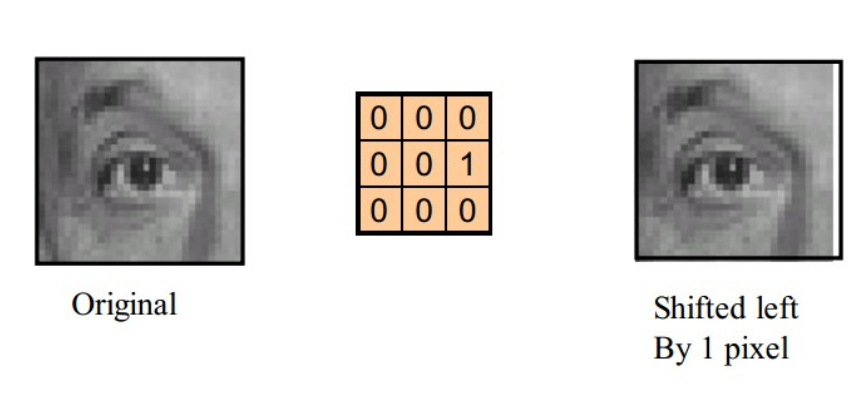
\includegraphics[height=150pt, keepaspectratio = true]{images/conv_easy4}   
	\end{figure}
\end{frame}

\begin{frame}\frametitle{Фильтр Гаусса}
	\begin{figure}[htbp]
	  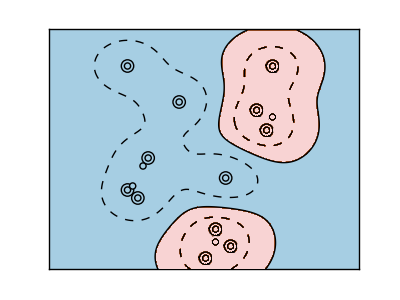
\includegraphics[height=150pt, keepaspectratio = true]{images/gauss}   
	\end{figure}
\end{frame}

\begin{frame}\frametitle{Подавление шумов}
	\begin{figure}[htbp]
	  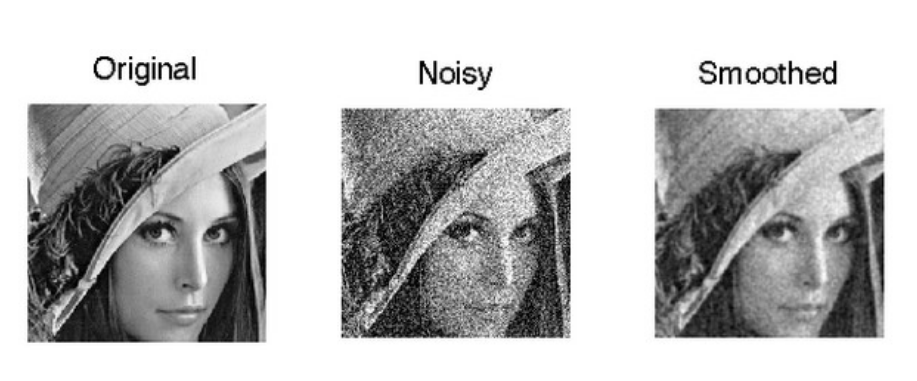
\includegraphics[height=130pt, keepaspectratio = true]{images/gauss2}   
	\end{figure}
\end{frame}

\begin{frame}\frametitle{Сверточный слой}
  Локально-связанный слой с одинаковыми весами в разных частях изображения.\\
  Закладывает в сеть априорное знание о том, что объект может встретиться в любой части изображения.
	\begin{figure}[htbp]
	  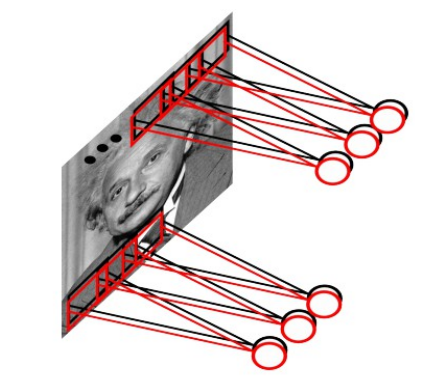
\includegraphics[height=180pt, keepaspectratio = true]{images/conv_layer}   
	\end{figure}
\end{frame}

\begin{frame}\frametitle{Subsampling слой}
	Добавляет устойчивости к небольшим деформациям.\\
	Max-subsampling аналогичен сверточному слою, в котором операция «+» заменена на «max»
	\begin{figure}[htbp]
	  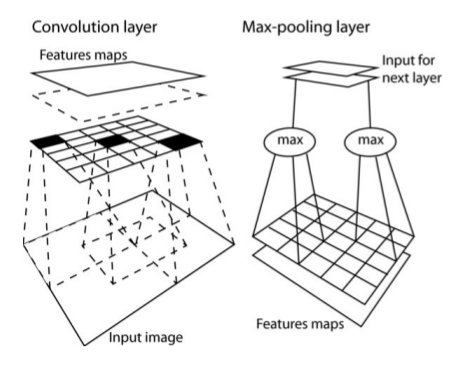
\includegraphics[height=180pt, keepaspectratio = true]{images/subsampling}   
	\end{figure}
\end{frame}

\begin{frame}\frametitle{Сверточная нейросеть}
	\begin{figure}[htbp]
	  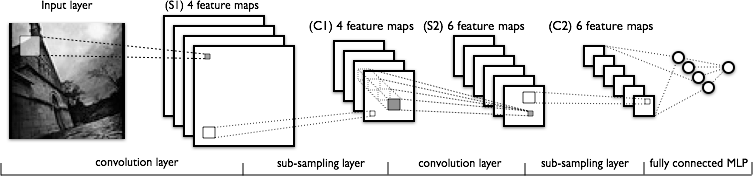
\includegraphics[height=75pt, keepaspectratio = true]{images/convnet}   
	\end{figure}
\end{frame}

\begin{frame}[standout]
  Вопросы?
\end{frame}

\appendix

\begin{frame}\frametitle{На следующей лекции}
	\begin{itemize}
    	\item[--] 
	\end{itemize}
\end{frame}

\end{document}
